\problem

\begin{captioneq}
	\centering
	\begin{align}
		\begin{split}
			A &=\begin{bmatrix}
				5.91  &-8.5914\\
				1.00  &                 0
			\end{bmatrix}\\
			B &=\begin{bmatrix}
				1\\0
			\end{bmatrix}\\
			C &= \begin{bmatrix}
				64.8 & 425.088
			\end{bmatrix}\\
			D &= \begin{bmatrix}
				0
			\end{bmatrix}
	\end{split}
	\end{align}
	\caption{State space model of plant.}
\end{captioneq}

\subproblem{Specifications}
\subsubsection*{Stability}
All poles and zeroes should be in the left half plane. For the state space matrices, eigenvalues of $A-BK<0$ and eigenvalues of $A-LC<0$.
\subsubsection*{Settling time}
The 2\% settling time must be no greater than 40\% that of the plant:
$$
t_{s.2\%} \leq 0.4 \SI{1.8333}{\second} = \SI{0.7333}{\second}
$$
I will aim for a 2\% settling time of \SI{0.7}{\second}. If the system is to behave as a first-order one with a dominant pole, that dominant pole must be to the left of $-\frac{4}{t_{s,2\%}}=-5.71$.

The plant has a zero at -6.806. To reduce the retarding effect of this zero I will introduce a pole near to it, at $p_1=-6.7$.

\subsubsection*{Percentage overshoot}
The plant's step response exhibits no overshoot. This specification then becomes that the closed loop step response must have a maximum of 25\% overshoot. This translates to a damping ratio $\zeta=0.4037$, I chose $\zeta=0.5$ (PO $\sim 16\%$) to give a margin. From the roots of the characteristic polynomial (below) we get two suggested poles of the system:
\begin{align*}
	&s^2+2\zeta \omega_n s + \omega_n^2,\qquad\omega_n=\frac{4}{\zeta t_{s,2\%}}\\
	s&=\num{-5.7143}\pm\num{9.8975j}
\end{align*}
To choose the above complex pair as poles would not allow me to satisfy the settling time specification with any margin|the real part of the pair is equal to the minimum magnitude requirement.

I will choose a pole at $p_2=-6$ to satisfy both the PO and $t_s$ requirements. The real pole should suppress oscillations and it is sufficiently negative that, were it dominant, the plant would be fast enough.


\subsubsection*{Steady state error}
The closed loop system must have zero steady state error to a step input. To this end a pre-amplifier is introduced to scale the reference input by a constant amount (K is the gain matrix defined in the next section):
\begin{align*}
	\bar{N} &= \frac{-1}{C(A-(B K))^{-1}B}
	&= 0.0955
\end{align*}

\subproblem{Introduced poles}
The poles of the plant are at $-3.378$ and $-2.838$. Both introduced poles are sufficiently negative to dominate these plant poles.
The gains such that the closed loop system has the introduced poles $\left\{-6.7,-6\right\}$ were found using \texttt{place}. The gains below are the  gains thus produced rounded up to the next integer gain:
$$
K = \left[7, 32\right]
$$

\subproblem{Observer}
\subsubsection*{Observer gain}
To implement the observer, first the gain of the difference between the system output and the observer output must be chosen. The aim is that the error reduce rapidly. As unnecessarily high gains should be avoided, I chose gains such as would introduce poles three times the greatest pole of the system as this appeared to produce acceptable results while not requiring very large gains. The simplified gains used are given below:
$$
L = \begin{bmatrix}
	2\\-0.3
\end{bmatrix}
$$
These were aimed to correspond to poles at $-21$ and $-22$.

\subsubsection*{State space model}
The matrices of the state space model of the closed loop system without the observer is given below:
\begin{align*}
	A &= \begin{bmatrix}
		  -12.91 &  -40.5914\\
		1 &  0
	\end{bmatrix}\\
B &= \begin{bmatrix}
	    0.0955\\
	0
\end{bmatrix}\\
C &= \begin{bmatrix}
	64.8 & 425.088
\end{bmatrix}\\
D &= \begin{bmatrix}
	0
\end{bmatrix}
\end{align*}
The matrices of the state space model of the system with the observer are given below:
\begin{align*}
	A &= \begin{bmatrix}
  -12.91 &  -40.5914  &  7 & 32\\
1     &    0    &     0    &     0\\
0    &     0 & -135.51 & -858.7674\\
0      &   0  &  20.44  & 127.5264\\
	\end{bmatrix}\\
	B &= \begin{bmatrix}
		0.0955\\
		0\\0\\0
	\end{bmatrix}\\
	C &= \begin{bmatrix}
		64.8 & 425.088 & 0 & 0
	\end{bmatrix}\\
	D &= \begin{bmatrix}
		0
	\end{bmatrix}
\end{align*}
\subproblem{Results}
\begin{figure*}
	\centering
	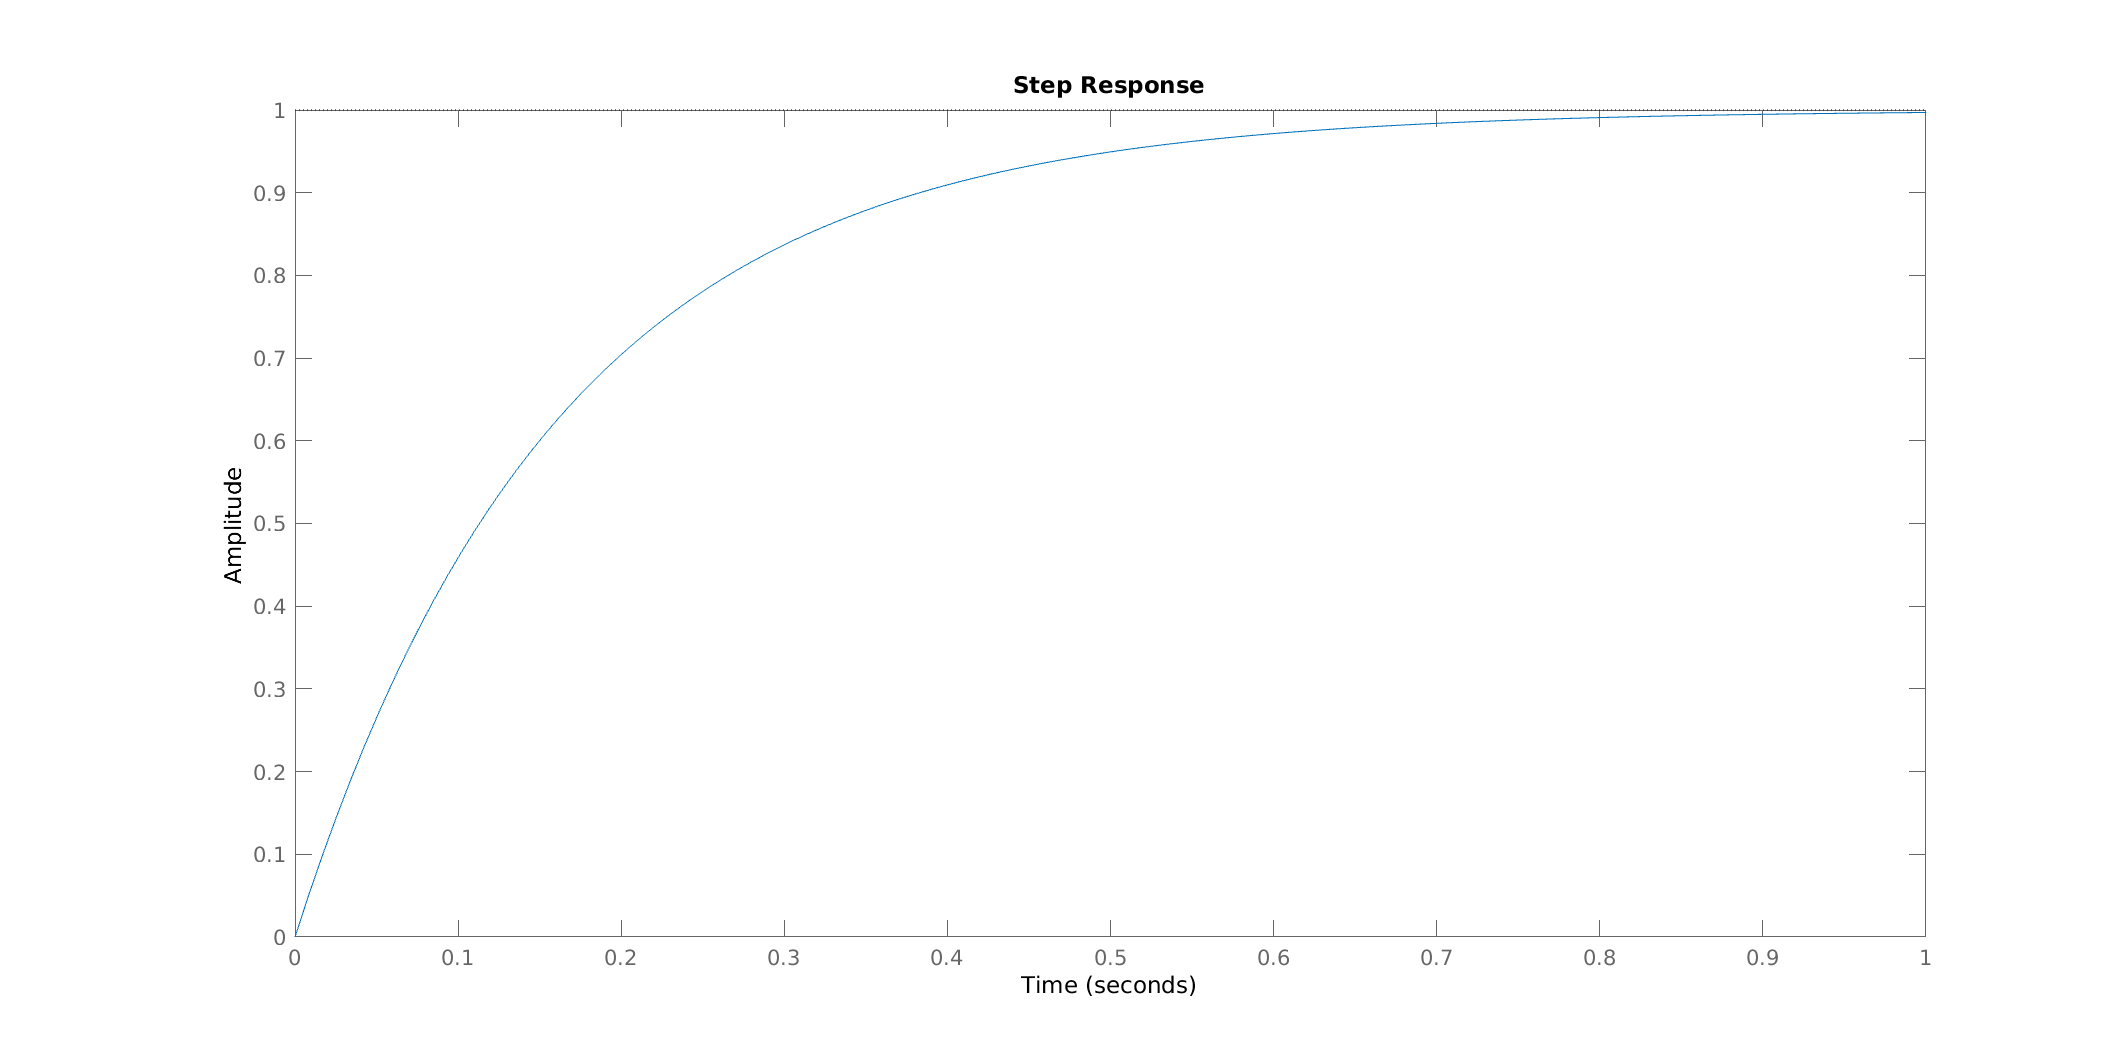
\includegraphics[width=\linewidth]{p3-step_observer.png}
	\caption{Step response of closed loop system with observer}
	\label{fig:p3:step Gcl observer}
\end{figure*}
\begin{table}[h]
	\centering
	\begin{tabular}{lr}
		\toprule
		Characteristic&Value\\
		\cmidrule(r){1-1}\cmidrule(l){2-2}
		Steady State Error & 0.07\%\\
		$t_{s,2\%}$ & \SI{ 0.6622}{\second}\\
		Overshoot & 0\%\\
		\bottomrule
	\end{tabular}
	\caption{Step characteristics of closed loop system}
	\label{tab:p3:step}
\end{table}
\Cref{fig:p3:step Gcl observer} gives the step response of the final closed loop system and \cref{tab:p3:step} some characteristics of the response.

All specifications have been met. The steady state error over the default \matlab time range is in the fourth decimal place and when the step response is extended goes to zero. All introduced poles have real magnitudes less than 0 so the system is stable.

\subsubsection*{Sensitivity to model parameters}
\ffigures{p3-sse_error.png/Steady state error./fig:p3:ts error,p3-ts_rel_err.png/Relative error in the 2\% settling time. Note that this is $\frac{t_s-t_{s,specified}}{t_{s,specified}}$./fig:p3:ts error}

\Cref{fig:p3:sse error} gives the magnitude of the error in the steady state value for deviations of $\pm 10\%$ in all parameters and \cref{fig:p3:ts error} gives the relative error in the 2\% settling time for the same deviations.

The range of the settling time was from 5.52\% below the specified value to 14.59\% below. The settling time specification was always met.

The steady state error ranged from 0.07\% to 16\%. 8\% of the deviations were under 1\%, 40\% of were under 5\% and 64\% were under 8\%. Whether or not this is acceptable depends on the application. One statistic that might be interesting also is that for the level of deviation of each individual parameter, 10\%, 78\% of the steady state errors were below this threshold.

The overshoot was 0 for all deviations, satisfying the specification.